\documentclass[11pt]{article}
\usepackage[margin=0.85in]{geometry}
\usepackage{booktabs}
\usepackage{microtype}
\usepackage{titling}
\usepackage{enumitem}
\usepackage{hyperref}
\usepackage{parskip}
\usepackage{amsmath}
\usepackage{graphicx}

\setlength{\droptitle}{-3.5em}
\setlist{nosep}
\hypersetup{hidelinks}

\title{Reproducing PatchTST on the ILI Benchmark}
\author{Cade Jin \quad Chenkai Shen \quad Derek Xu \\
        Cornell University \quad CS 4782 (Spring 2026) \\
        \small Code: \url{https://github.com/Derek-Cornell/Project}}
\date{\vspace{-1.5em}}

\begin{document}
\maketitle
\vspace{-2.5em}

\section*{1. Introduction}
For years, Transformer-based time series forecasters underperformed simple linear baselines. The culmination was DLinear (Zeng et al., AAAI 2023), a single linear layer that beat every prior Transformer forecaster. PatchTST (Nie et al., ICLR 2023) finally flipped this. Instead of tokenizing each timestep, they group consecutive timesteps into \emph{patches} as tokens. Each patch encodes a meaningful sub-trajectory rather than a single noisy observation, giving attention something semantically richer to operate on. They also run the Transformer on each channel independently. With those two changes, PatchTST beats DLinear across the board.

We reproduce that claim on ILI, the smallest benchmark in the paper, and add an ablation the paper does not include. PatchTST uses a \emph{direct} head, a single linear layer of output dimension $T$. We swap it for an \emph{autoregressive} (AR) head that emits one patch at a time and rolls forward $\lceil T/P\rceil$ times. We expected AR to be at a disadvantage from compounding errors and exposure bias, with a possible parameter-efficiency upside. AR's head stays the same size regardless of $T$ while direct's grows linearly with horizon, which can matter on small datasets where the direct head has more parameters than training samples.

\section*{2. Chosen Result}
We target the ILI rows of \textbf{Table 3} of Nie et al., comparing supervised PatchTST against DLinear at horizons $T \in \{24, 36, 48, 60\}$ weeks with look-back $L = 104$. We initially started with Electricity but a single training run took close to two hours on the A100, and the autoregressive head was projected to run much slower since it calls the encoder once per rollout. To iterate fast on the AR ablation, we switched to ILI, the smallest benchmark in the paper ($n{=}966$ weekly samples, 7 channels), where a full multi-seed sweep runs in minutes per horizon.

\section*{3. Methodology}
\textbf{Re-implementation.} We rebuilt PatchTST and DLinear from scratch in PyTorch. PatchTST uses channel-independence, patching with $P{=}24, S{=}2$ (92\% overlap, 42 tokens), a 3-layer Transformer encoder with BatchNorm and residual attention, $d_{\text{model}}{=}16$, $H{=}4$ heads, $d_{\text{ff}}{=}128$, dropout 0.3, and RevIN (\texttt{affine{=}False}). DLinear uses the standard moving-average decomposition with a \texttt{Linear}$(L \to T)$ per component, summed. Both apply the standard 70/10/20 chronological split with \texttt{StandardScaler} fit on training data only. We verified our PatchTST against the source by copying weights across and confirming max abs diff $= 0.0$ in direct mode.

\textbf{Training.} Adam, MSE, batch 16, lr $2.5\!\times\!10^{-3}$ constant, 100 epochs. PatchTST runs on 3 seeds $\{1, 42, 2021\}$ in both direct and AR modes; DLinear is single-seed.

\textbf{The autoregressive head.} Direct's head is \texttt{Linear}$(N{\cdot}D \to T)$, with 16k parameters at $T{=}24$ and 40k at $T{=}60$ on ILI. The AR head outputs one patch ($P{=}24$ values) regardless of $T$, fixing its parameter count at 16k. To predict longer, we append the prediction to the look-back, drop the oldest 24 timesteps, re-encode, and emit the next patch, repeating $\lceil T/P \rceil$ times. The encoder, patching, and RevIN are unchanged. Training is end-to-end with autograd flowing back through every rollout.

\section*{4. Results \& Analysis}

\begin{table}[h]
\centering\small
\begin{tabular}{lrrrrrrr}
\toprule
Model & $T$ & Ours MSE & Paper MSE & $\Delta$ MSE & Ours MAE & Paper MAE & $\Delta$ MAE \\
\midrule
PatchTST direct & 24 & $1.577 \pm 0.124$ & 1.319 & $+0.26$ & $0.823 \pm 0.041$ & 0.754 & $+0.07$ \\
PatchTST AR     & 24 & $1.577 \pm 0.124$ & ---   & ---    & $0.823 \pm 0.041$ & ---   & ---    \\
PatchTST direct & 36 & $1.561 \pm 0.113$ & 1.430 & $+0.13$ & $0.854 \pm 0.022$ & 0.834 & $+0.02$ \\
PatchTST AR     & 36 & $1.645 \pm 0.129$ & ---   & ---    & $0.862 \pm 0.056$ & ---   & ---    \\
PatchTST direct & 48 & $1.715 \pm 0.067$ & 1.553 & $+0.16$ & $0.876 \pm 0.047$ & 0.815 & $+0.06$ \\
PatchTST AR     & 48 & $1.800 \pm 0.074$ & ---   & ---    & $0.895 \pm 0.026$ & ---   & ---    \\
PatchTST direct & 60 & $1.913 \pm 0.221$ & 1.470 & $+0.44$ & $0.959 \pm 0.063$ & 0.788 & $+0.17$ \\
PatchTST AR     & 60 & $1.704 \pm 0.091$ & ---   & ---    & $0.902 \pm 0.032$ & ---   & ---    \\
\midrule
DLinear & 24 & 1.905 & 2.215 & $-0.31$ & 0.967 & 1.081 & $-0.11$ \\
DLinear & 36 & 2.147 & 1.963 & $+0.18$ & 1.025 & 0.963 & $+0.06$ \\
DLinear & 48 & 2.171 & 2.130 & $+0.04$ & 1.037 & 1.024 & $+0.01$ \\
DLinear & 60 & 2.340 & 2.368 & $-0.03$ & 1.089 & 1.096 & $-0.01$ \\
\bottomrule
\end{tabular}
\caption{\small Test MSE/MAE on ILI. PatchTST is mean $\pm$ std over 3 seeds, DLinear is single-seed, and $\Delta$ = ours $-$ paper. Paper has no AR baseline. $T{=}24$ AR equals direct by construction (one rollout). PatchTST beats DLinear at every horizon by 0.33--0.59 MSE.}
\end{table}

\vspace{-0.5em}
\textbf{Reproduction.} PatchTST beats DLinear at every horizon, matching the paper's central claim, and our DLinear tracks the paper's within $\pm 0.31$ MSE. Our PatchTST means come in 0.13--0.44 MSE higher than the paper's, with the $T{=}60$ gap at roughly $2\sigma$ of our seed variance. We attribute the residual to the paper's single-seed reporting on a 966-row dataset plus small undocumented training-pipeline details.

\begin{figure}[t]
    \centering
    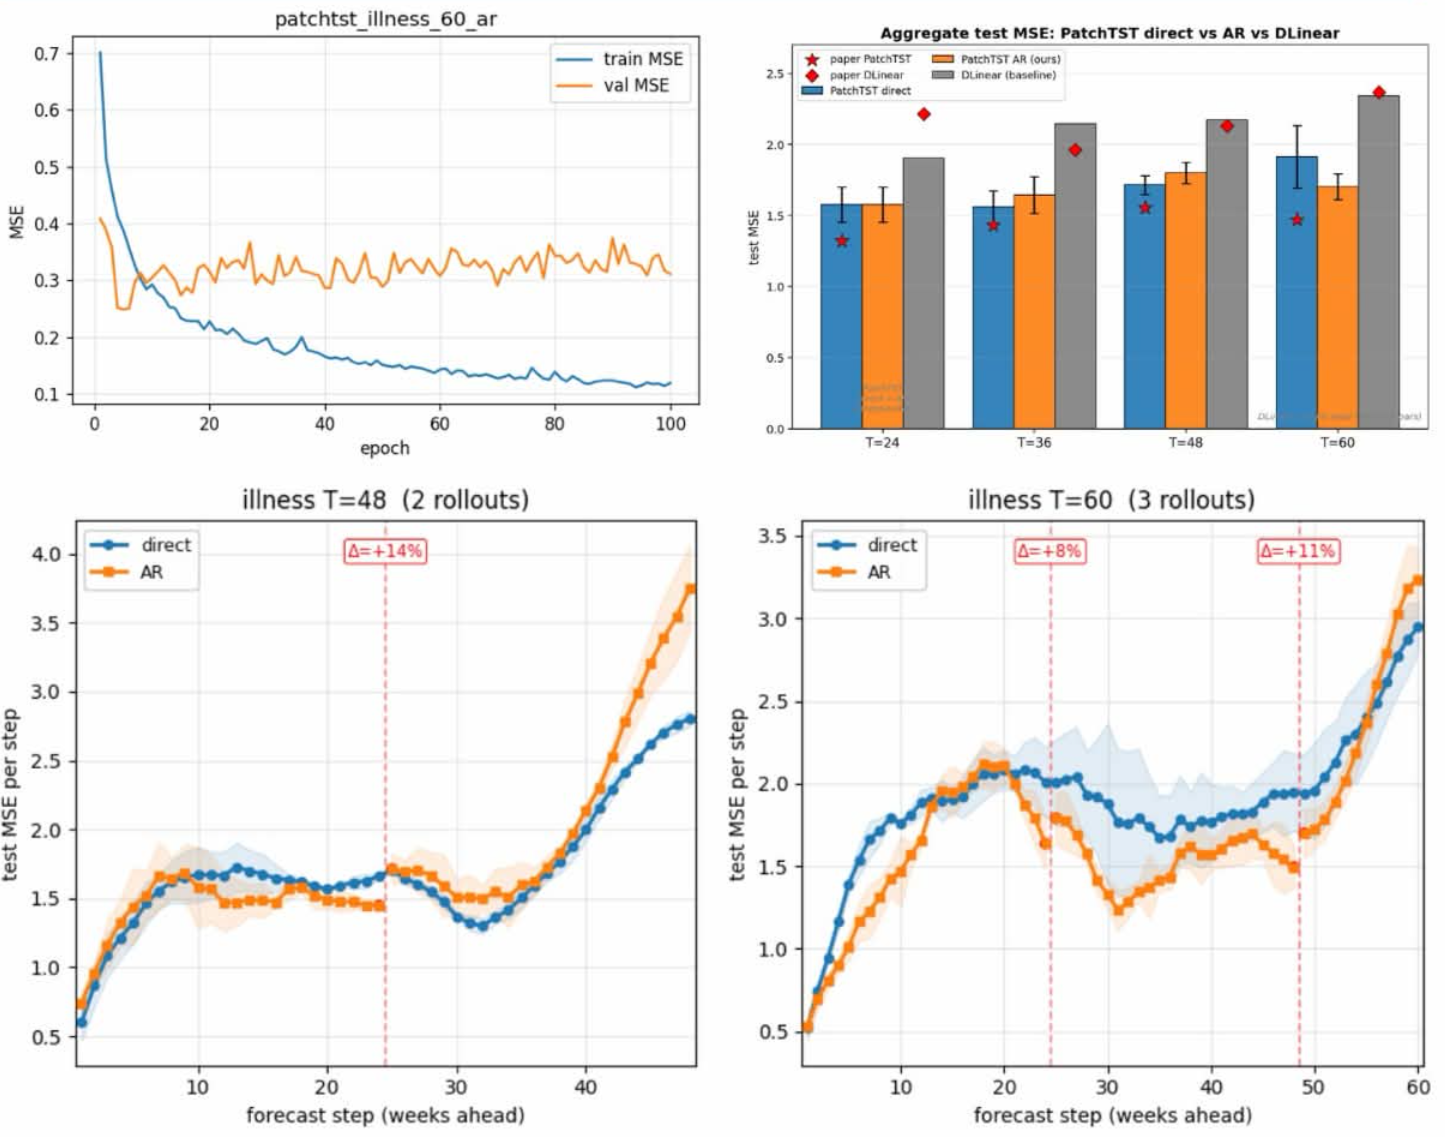
\includegraphics[width=0.85\linewidth]{DL graphs.png}
    \caption{\small Autoregressive PatchTST on ILI. Top: training/validation MSE at $T{=}60$ and aggregate test MSE across horizons. Bottom: per-step test MSE for direct vs.\ AR at $T{=}48$ and $T{=}60$ with $\pm 1\sigma$ bands. Discontinuities in AR's curve at every 24-step rollout boundary are the exposure-bias signature.}
    \label{fig:ar_direct_per_step}
\end{figure}

\textbf{Direct vs.\ autoregressive head.} At $T{=}24$, AR equals direct by construction (one rollout). At $T{=}36$ and $T{=}48$, AR is slightly worse on point estimate (paired $\Delta \approx +0.08$ MSE) with overlapping bands, a tie. At $T{=}60$, AR's aggregate mean is 0.21 MSE below direct's, with paired $\Delta = -0.21 \pm 0.14$ across 3 seeds, suggestive but only $\sim 1.5\sigma$ and plausibly flippable with more seeds.

The per-step decomposition in Figure~\ref{fig:ar_direct_per_step} clarifies what aggregate MSE alone hides.

\textbf{(1) Exposure-bias spikes appear at every rollout boundary.} Direct's error grows smoothly while AR's jumps discontinuously where the rollout transitions from real ground-truth to ``real plus the model's own predictions.'' At $T{=}48$, AR's MSE jumps $+0.26$ at step 25 while direct's rises by $+0.04$. At $T{=}60$, AR jumps $+0.15$ at step 25 and $+0.20$ at step 49 while direct is essentially flat. The exposure-bias cost we expected is real and mechanistically clean.

\textbf{(2) AR is worse than direct at the end of $T{=}60$.} AR is better in the middle (steps 25--48, up to 30\% relative) but worse in the last 5 steps (56--60, by 4--11\%). By the third rollout, nearly half the context is synthetic and accumulated errors dominate. The aggregate $T{=}60$ ``win'' is won by middle-horizon gains, not by better far-horizon prediction.

\textbf{(3) The middle-horizon AR advantage coincides with direct's variance balloon.} Direct's $\pm 1\sigma$ band widens to $\sim 1.0$ MSE units in the middle while AR's stays around 0.3. Where AR appears to win is exactly where one or two unlucky direct seeds could pull its mean up, so we cannot cleanly distinguish a systematic AR advantage from seed noise. AR's std at $T{=}60$ is 0.091 vs.\ direct's 0.221, a 2.4$\times$ tighter distribution and the clearest robust finding.

\textbf{Takeaway.} AR pays the predicted exposure-bias cost, aggregate MSE is tied or noisily in AR's favor, and AR's lower seed-to-seed variance is the cleanest robust finding.

\section*{5. Reflections}
\textbf{Lessons.} Seed variance dominates on small datasets. Our 3-seed std at $T{=}60$ is 0.22 MSE, half the gap between our mean and the paper's. The qualitative ranking (PatchTST beats DLinear) is durable, but precise numbers are noisier than they look. Single-seed runs flattered us early. PatchTST/$T{=}24$ at seed 2021 gave 1.418 MSE near the paper's 1.319, but the 3-seed mean was 1.577. Most importantly, aggregate metrics mislead even with multi-seed averaging. Our $T{=}60$ paired $\Delta$ looked like a small AR win until the per-step view showed the advantage was concentrated where direct's variance is large and that AR is actually worse in late-horizon steps. The general lesson is that visualizing along the axis where the architecture differs, here the time axis, is essential for any architectural ablation.

\textbf{What we'd do differently.} Allocate the seed budget before the ablation budget. Several early conclusions flipped after multi-seed sweeps. We would also run DLinear on the same seeds as PatchTST to control for run-to-run noise on both sides of the table.

\textbf{Future work.} The natural next step is to repeat the AR ablation on Electricity and Traffic, which have $\sim 30\times$ more training data, to test whether the rollout-boundary spikes persist outside small-data regimes. The AR head should also be tried at $T \gg P$ such as Electricity $T{=}720$, where direct's head has nearly 4M parameters in just the output layer. Standard exposure-bias mitigations such as scheduled sampling could shrink the boundary spikes without giving up AR's fixed-parameter-count advantage. A per-channel breakdown of test MSE would also clarify which of the 7 ILI variables drives the aggregate result.

\section*{References}
\small
[1] Nie, Y., Nguyen, N.H., Sinthong, P., Kalagnanam, J. \textit{A Time Series is Worth 64 Words: Long-Term Forecasting with Transformers.} ICLR 2023. arXiv:2211.14730. \\

[2] Zeng, A., Chen, M., Zhang, L., Xu, Q. \textit{Are Transformers Effective for Time Series Forecasting?} AAAI 2023. arXiv:2205.13504. \\

[3] AI assistance disclosure: Our group used ChatGPT and Claude for help with understanding the original papers, developing/debugging the PyTorch re-implementations of PatchTST and DLinear, and editing the autoregressive extension and final report.

\end{document}
